\documentclass[12pt]{article}
\usepackage{geometry}
\geometry{a4paper}


\usepackage{color}
\usepackage{hyperref}
\usepackage{amsmath}
\usepackage{amsfonts}
\usepackage{amssymb}
\usepackage{graphicx}
\usepackage{tcolorbox}
\usepackage{listings}
\usepackage{here}
\usepackage{txfonts}
\usepackage{algorithm}
\usepackage{algorithmic}
\usepackage{siunitx}
\usepackage{xcolor}

\lstset {language = c++,
  basicstyle = \ttfamily \scriptsize,
  commentstyle = \textit,
  frame = tRBl,
  framesep = 5pt,
  showstringspaces = false,
  numbers = left,
  stepnumber = 1,
  numberstyle = \tiny,
  tabsize = 2,
  keywordstyle = \bfseries \color{blue},
  stringstyle=\color{magenta},
  commentstyle=\color{red},
  morecomment=[l][\color{red}]{\#}
  showstringspaces=false, % don't mark spaces in strings
}
\newcommand{\bi}[1]{\mathbf{#1}}
\newcommand{\bs}[1]{\boldsymbol{#1}}  % bold for greek characters
\newcommand{\bbR}{\mathbb{R}}

\author{Nobuyuki Umetani}

\title{Parametric Curve}


\begin{document}
\maketitle
\tableofcontents


\section{Parametric Curve}


Arc-length:
\begin{eqnarray}
\int_0^1 \sqrt{ \left( \frac{d\bi{p}}{dt}(t) \right)^2 } dt \\
\end{eqnarray}

Tangent
\begin{equation}
\frac{d\bi{p}}{dt}
\end{equation}

\section{Bezier Curve}

\begin{equation}
\bi{p}(t) = (1-t)^3\bi{p}_0 + 3(1-t)^2t\bi{p}_1 + 3(1-t)t^2\bi{p}_2 + t^3\bi{p}_3
\end{equation}

Tangent

\begin{equation}
\frac{d\bi{p}}{dt}(t) = -3(1-t)^2\bi{p}_0 + 3(3t-1)(t-1)\bi{p}_1 - 3t(3t-2)\bi{p}_2 + 3t^2\bi{p}_3
\end{equation}




\subsection{De Casteljau's algorithm}




\section{B-Spline Curve}


B-Spline curve is constructed from the three ingredients. 
\begin{itemize}
\item the degree of the polynominal basis $p$.
\item a set of $n$ control points $\{\bi{p}_0,\ldots, \bi{p}_{n-1}\}$,
\item a knot vector $\bi{u}$ of $m+1$ non-descending real number $\{u_0\le u_1 \le  u_2\ldots \le u_{m}\}$ where $m=n+p$.
\end{itemize}
%
It is a bit confusing but, if the basis is $p$ degree polynominal, the B-Spline curve is called $p+1$ order.
%
The order of the B-Spline means that up to $p+1$ control points affects a position of a point on the curve.

%
From the knot vector and $p$, we can define a basis function $N_{i,p}(u)$ which takes value in the range $u\in [u_0,u_m]$.
%
Then, the resulting equation of the curve becomes
%
\begin{equation}
\bi{p}(u) = \sum_{i=0}^{n-1} N_{i,p}(u)\bi{p}_i
\end{equation}


\subsection{Knot Vector}

The knot vector $\bi{u}$ defines segments on the parameter the curve.
%
This allows non-uniformly sized segments and gives the B-Spline higher degree of expression.
%
Quite frequently, the interval between knots become zero $0$ if the knot takes the same value.
%
The number of the time the knot duplicate is called \textit{knot’s multiplicity}.



\subsection{Cox - De Boor's algorithm}

The basis function is defined hierarchically. 
%
In other words, we build up the basis function based on the basis function of one order lower.


We start from $0$ degree basis function which is piecewise constant over the interval
%
\begin{equation}
N_{i,0} (u)
= \left\{ \begin{array}{rl}
1 & if \; u_i < u < u_{i+1} \\
0 & otherwize
\end{array}\right.
\end{equation}
%
Then, for $p>0$, we define the basis functions using the basis function of $p-1$ degree as
%
\begin{equation}
N_{i,p}(u) = 
\frac{u-u_{i}}{u_{i+p}-u_i} N_{i,p-1}(u)
+ 
\frac{u_{i+p+1}-u}{u_{i+p+1}-u_{i+1}} N_{i+1,p-1}(u)
\label{eqn:deboor}
\end{equation}

Figure~\ref{fig:deboor_basis} show the basis functions of the B-Spline with different degrees. 
%
Please notice that, \textcolor{red}{the degree $p$ basis functions have a domain of $p+1$ intervals}.
%
So if you go up in the higher degree, the influence of a control point gets wider, meaning that the function become smoother. 
%
Further more, given a parameter $t\in [t_0,t_m]$, it will cover by up to $p+1$ basis function.
%
This means that \textcolor{red}{$p+1$ control points influence a point on the B-Spline curve}.

\begin{figure}[htbp!]
\center
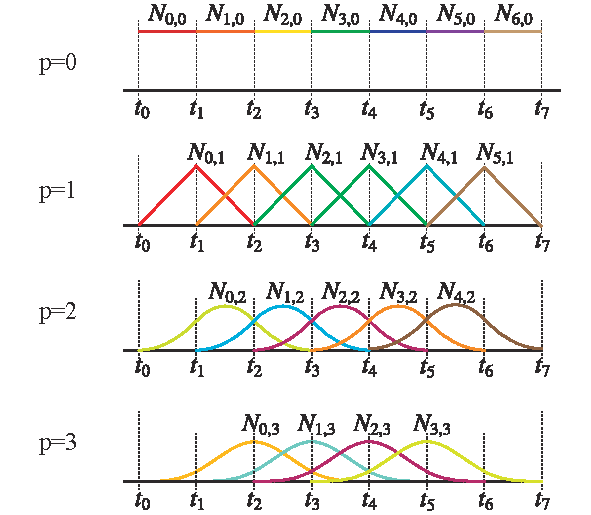
\includegraphics[width=100mm]{images/deboor_basis.pdf}
\caption{Basis functions of a B-Spline curve with uniform knots. The degree of the basis function increases from top row ($p=0$) to be bottom row ($p=3$). }
\label{fig:deboor_basis}
\end{figure}



Figure~\ref{fig:deboor_operation} shows that example of the B-Spline basis function construction from the basis functions of $p=1$ to one of $p=2$ using the \eqref{eqn:deboor}.
%
Starting from two neighboring basis functions we call left and right functions, we multiply a linear functions for each.
%
For the left basis function we multiply a linear function that goes from zero to one over the domain of the function. 
%
Domain of the function means where the function takes value other than zero. 
%
In this case $p=1$ functions takes two segments as the domain.
%
Similarly, we multiply the right basis function to a linear function that linearly goes down from one to zero over its domain.
%
If we multiply a linear function to $p$ degree function, we get a $p+1$ degree function. 
%
Adding up these two functions, we get a new basis. 
%
Because the left and right basis function have domains different by one segment, the new basis function gets a one segment wider. 





\begin{figure}[htbp!]
\center
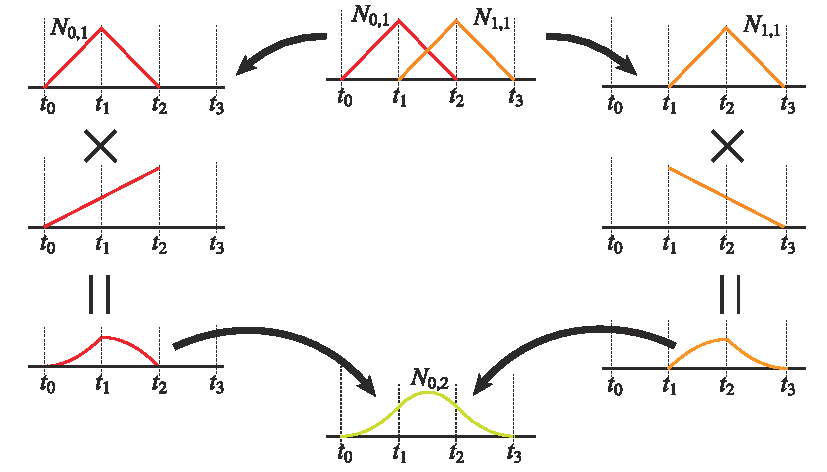
\includegraphics[width=140mm]{images/deboor_operation.pdf}
\caption{Cox - De Boors algorithm applied to two neighboring piece-wise linear basis functions to produce a piece-wize quadratic basis function.}
\label{fig:deboor_operation}
\end{figure}


\subsection{Knot Insertion}

We can insert a knot in the knot vector without changing the curve shape.



Let's say we insert a knot $u$ in the knot vector.
%
Because the knot values need to be monotonically increase, the $u$ need to be insert in the interval $[u_k,u_{k+1}]$ where $ u_k\le  u \le u_{k+1}$.
%
If we add one knot value, one control point need to be added (remember the relation $n=m+p$).
%
There are $p+1$ number of basis functions whose domain include $u$ are $N_{k-p,p},\ldots,N_{k,p}$.
%
Hence by the knot insertion only the corresponding control points $\bi{p}_{k-p},\ldots,\bi{p}_k$ need to be considered. 

 



\begin{figure}[htbp!]
\center
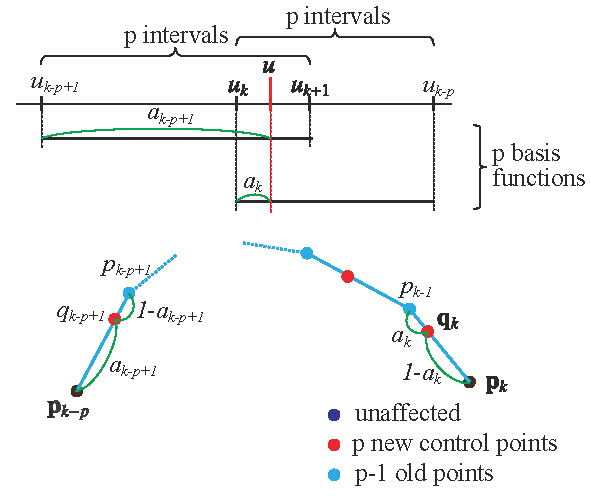
\includegraphics[width=100mm]{images/deboor_insert.pdf}
\caption{knot insertion algorithm}
\label{fig:deboor_insert}
\end{figure}

De Boor's algorithm says the new control point locations are on the polyline connecting the old control points.
%
$p-1$ number of old control points $\bi{p}_{k-p+1},\ldots,\bi{p}_{k-1}$ are replaced by $p$ number of new control points $\bi{q}_{k-p+1},\ldots,\bi{q}_k$.
%
For example, the new control point $\bi{q}_i$ lies on the line segment connecting $\bi{p}_{i-1}$ and $\bi{p}_i$.  

\begin{align}
\bi{q}_i &= (1-a_i) \bi{p}_{i-1} + a_i\bi{p}_i\;\;\;\;  \; (k-p+1 \le i \le k) \\
where \;\;\; a_i      &=  \frac{u-u_i}{u_{i+p}-u_i} 
\end{align}



\subsection{Evaluation of a Point}




\section{NURBS Curve}
%
The NURBS is the abbreviation of \underline{N}on-\underline{U}niform \underline{R}ational \underline{B}-\underline{S}pline curve. 
%
``non-uniform" means that the interval of the knots can be uneven. 
%
Rational means there are weight $w$ for the control points.
%
\begin{equation}
\bi{p}(u) = \frac{\sum_{i=0}^{n-1} N_{i,p}(u)w_i\bi{p}_i}{\sum_{i=0}^{n-1} N_{i,p}w_i }
\end{equation}
%
This weight gives further control ability to the curve. 


Each control points have a weight $w_i$. 
%
If all the weight is $1$ it becomes a B-Spline curve with non-uniform knot interval.
%






\subsection{How NURBS can Represent a Perfect Circle}


Let's use a homogeneous coordinate to understand how the NURBS can successfully define a perfect circle. 
%
Here we think about two dimensional space where.
%
A homogenious coordinate has additional one dimension $w$ in addition to the $xy$.
%
The point $(x,y,w)$ in homogeneous coordinate corresponds to the two dimensional point $(x/w,y/w)$.
%
Such a homogeneous coordinate is called Affine transformation and is very useful in computer graphics to define perspective transformation.
%


\begin{figure}[htbp!]
\center
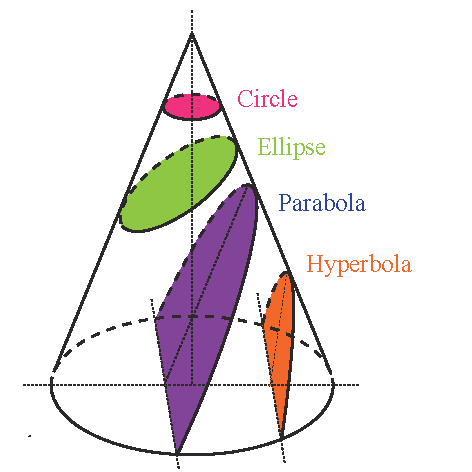
\includegraphics[width=80mm]{images/cone.pdf}
\end{figure}






\begin{figure}[htbp!]
\center
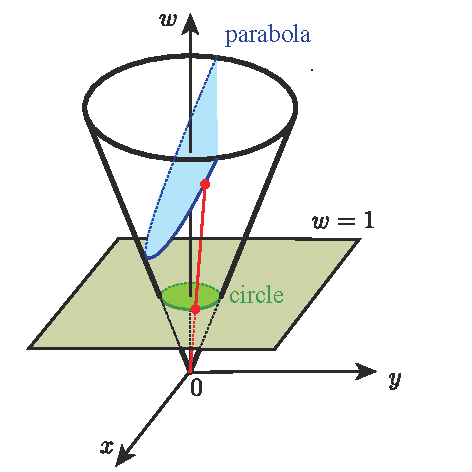
\includegraphics[width=80mm]{images/parabola.pdf}
\end{figure}



\begin{eqnarray}
u_0,u_1,u_2,u_3,u_4,u_5,u_6,u_7\\
0,x,y,w,w=1\\
\bi{p}_{k-p-1},\bi{p}_{k-p},\bi{p}_{k},\bi{p}_{k+1}\\
\bi{q}_{k-p-1},\bi{q}_{k-p},\bi{q}_{k},\bi{q}_{k+1}
\end{eqnarray}






\end{document}
